\begin{enumerate}[label=\thesubsection.\arabic*.,ref=\thesubsection.\theenumi]
    \numberwithin{equation}{enumi}
    \numberwithin{figure}{enumi}

    \item A series-shunt feedback amplifier employs a basic amplifier with input and output resistances each of $2K\Omega$ and
    gain G = 1000V/V. The feedback factor H = 0.1V/V. Find the input resistance $R_{if}$, output resistance $R_{of}$ and gain 
    of the closed-loop amplifier. \\
    
\solution 
For given data, see Table:\ref{table:ee18btech11039_tab1}.
For feedback-amplifier circuit and equivalent circuit, see fig:\ref{fig:ee18btech11039_fig1} and \ref{fig:ee18btech11039_fig2}

\begin{table}[!h]
\centering
\input{./tables/ee18btech11039/ee18btech11039_tab1.tex}
\caption{}
\label{table:ee18btech11039_tab1}
\end{table}

\begin{figure}[!h]
		\resizebox{\columnwidth}{!}{\input{./figs/ee18btech11039/fig1.tex}}
\caption{Ideal structure}
\label{fig:ee18btech11039_fig1}
\end{figure}

\begin{figure}[!h]
		\resizebox{\columnwidth}{!}{\input{./figs/ee18btech11039/fig2.tex}}
\caption{Equivalent circuit}
\label{fig:ee18btech11039_fig2}
\end{figure}

Closed-loop gain,
\begin{align}
    T = \frac{G}{1+GH}
      = 9.9
\end{align}

\text{Input resistance,}
\begin{align}
    R_{if} = \brak{1+GH} R_i
    = 202K\Omega
\end{align}

\text{Output resistance,} 
\begin{align}
    R_{of} = \frac{R_o}{1+GH}
           = 19.802\Omega
\end{align}

\begin{figure}[!h]
		\resizebox{\columnwidth}{!}{\input{./figs/ee18btech11039/fig3.tex}}
\caption{Amplifier design}
\label{fig:ee18btech11039_fig3}
\end{figure}

\begin{figure}[!h]
		\resizebox{\columnwidth}{!}{\input{./figs/ee18btech11039/fig4.tex}}
\caption{G circuit}
\label{fig:ee18btech11039_fig4}
\end{figure}

\begin{figure}[!h]
		\resizebox{\columnwidth}{!}{\input{./figs/ee18btech11039/fig5.tex}}
\caption{H circuit}
\label{fig:ee18btech11039_fig5}
\end{figure}

\begin{table}[!h]
\centering
\input{./tables/ee18btech11039/ee18btech11039_tab2.tex}
\caption{Parameter values}
\label{table:ee18btech11039_tab2}
\end{table}

From fig:\ref{fig:ee18btech11039_fig4}
\begin{align}
G = \mu \frac{R_L || \brak{R_1 + R_2}}{\sbrak{R_L || \brak{R_1 + R_2}}+r_o} \frac{R_{id}}{R_{id}+R_s+\brak{R_1||R_2}} = 1000
\end{align}

Open-loop input resistance,
\begin{align}
     R_i =  R_s + R_{id} + \brak{R_1 || R_2} = 2K\ohm
\end{align}

From fig:\ref{fig:ee18btech11039_fig5}
\begin{align}
H = \frac{V_f}{V_o} = \frac{R_1}{R_1 + R_2} = 0.1
\end{align}

Open-loop output resistance,
\begin{align}
      R_o = r_o || R_L || \brak{R_2 + R_1} = 2K\ohm
\end{align}


\begin{figure}[!h]
		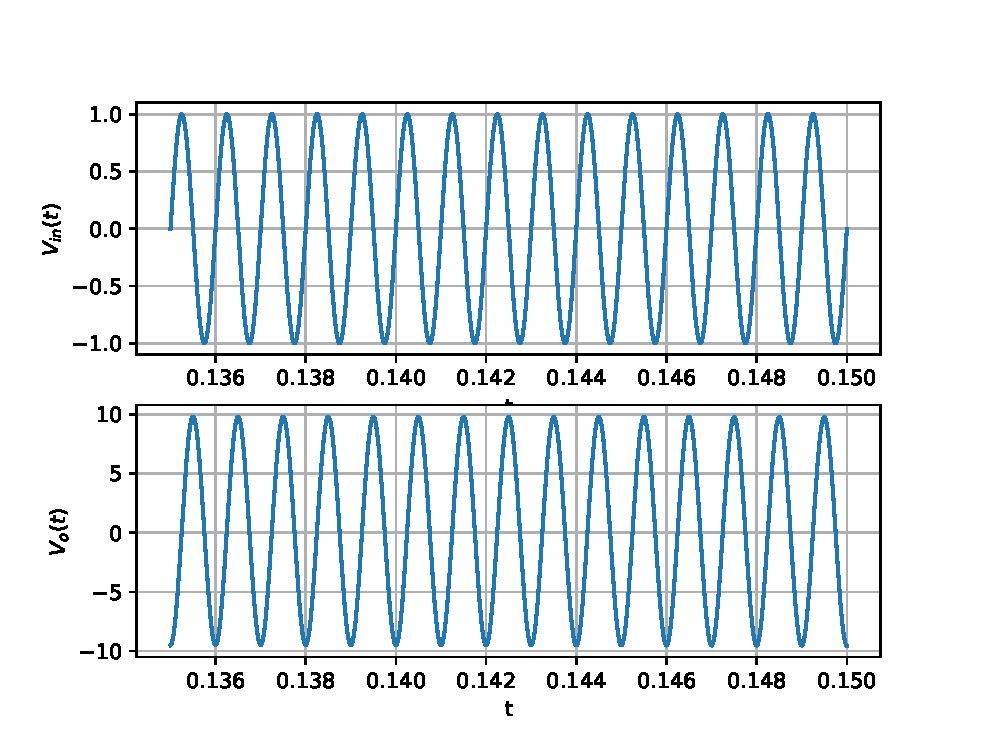
\includegraphics[width=\columnwidth]{./figs/ee18btech11039/spice_1.eps}
\caption{Steady-state output of the simulation}
\label{fig:ee18btech11039_fig6}
\end{figure}

\end{enumerate}